% !TEX root = flow_head.tex
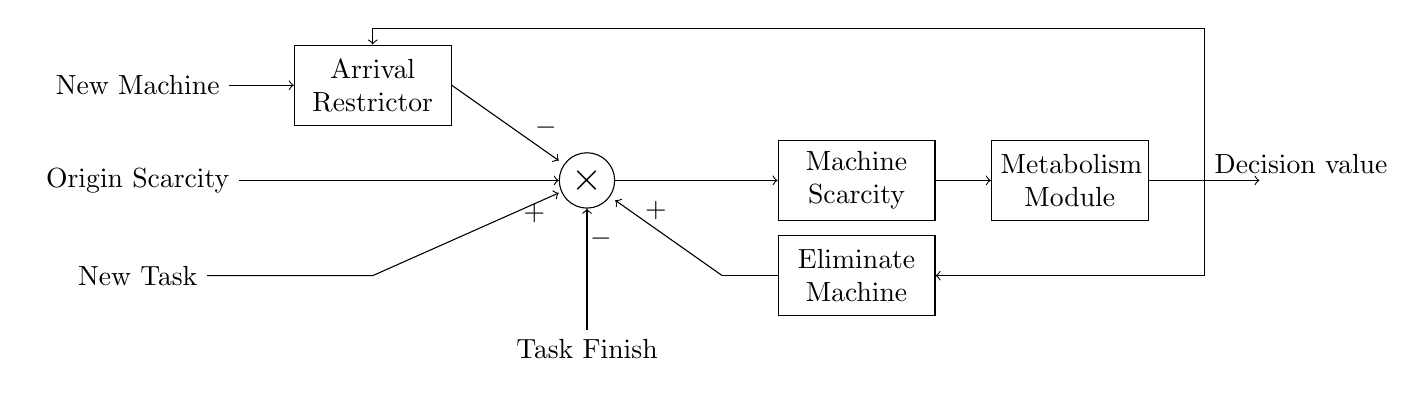
\begin{tikzpicture}[node distance=5mm and 5mm,
square/.style={
% The shape:
rectangle,
draw=black,
minimum size=2.9em,
text width=5em,
text centered
},
coord/.style={
coordinate,
% on chain,
% on grid,
% node distance=6mm and 25mm
},
circle/.style={
rectangle,minimum size=2em,rounded corners=1em,
draw=black
},
skip loop/.style={to path={-- ++(0,#1) -| (\tikztotarget)}}
]
\matrix[row sep=0.5em,column sep=2em] {
% First row:
\node (add) {New Machine}; & \node (machinein) [square] {Arrival Restrictor}; & & & & & & &\\
\node (origin) {Origin Scarcity}; & & \node (compare) [circle] {\Large$\times$}; & & \node (scarcity) [square] {Machine Scarcity}; & \node (metabolism) [square] {Metabolism Module}; &\node (node) [coord] {}; &\node (end) [coord] {};\\
\node (task) {New Task}; & \node (p1) [coord] {};& & \node (p2) [coord] {}; & \node (reduce) [square] {Eliminate Machine}; & & & & \\
& & \node (tf) {Task Finish}; &  & & & & &\\
};
\path (add) edge[->] (machinein) (machinein.east) edge[->] (compare) (compare) edge[->] (scarcity) (scarcity) edge[->] (metabolism);
\path (origin) edge[->] (compare);
\path (tf) edge[->] (compare);
\path (reduce) edge (p2) (p2) edge[->] (compare);
\draw [->] (metabolism) -- (end) ;
\draw [->]  (task) -- (p1) -- (compare);
\path (node) edge[->,skip loop=5.5em] (machinein);
\draw [->] (node) |- (reduce);
\path (machinein.east) to node [near end,yshift=0.5em,xshift=0.5em] {$-$} (compare);
\path (tf) to node [near end,xshift=0.5em] {$-$} (compare);
\path (p1) to node [near end,xshift=0.8em] {$+$} (compare);
\path (p2) to node [near end,xshift=0.5em,yshift=0.3em] {$+$} (compare);
\path (node) to node [near end,xshift=2em,yshift=0.6em] {Decision value} (end);
\end{tikzpicture}